\section{Challenges Of \spath Caching}\label{sec:competitors}

In this section we qualify the differences between static (no change in cache content at service runtime) and dynamic caching (Cache content is changed at service runtime) of \spathsns. We also introduce our state of the art competitor and explain why it is not an adequate solution for the \spath caching problem.


Using a dynamic cache\footnotemark and calculating the utility of each path is very expensive. If a dynamic cache is used, and we want to ensure it always keeps the most useful paths in the cache, it will be very expensive to calculate the utility of a new query with respect how much it overlaps with existing \spaths (i.e. how many vertices it shares with an existing \spathns) and how likely it will be able to answer a query in the future, thus adding a substantial overhead to query processing. As the utility of a \spath is so expensive to calculate, while the \spath service is running, it violates goal \ref{item:goal2} in section \ref{subsec:goals}.

Using \lru as the cache replacement policy in a dynamic cache ensures that only minimal overhead is added by using a dynamic cache. When a new query is submitted \lru evicts the least recently used \spath and keeps the most recently used \spaths in the cache.
\lru, however, has several shortcomings: 
\begin{itemize}
\item It has no way to determine the usefulness of inserting a path (i.e. no scoring function), which violates goal \ref{item:goal3} (Sec. \ref{subsec:goals}). Because \lru does not have a scoring function then, even if a path $P$ is valuable (covers many potential queries), if a sequence of consecutive queries, which $P$ can not cover, is submitted, then P will be evicted. 
\item \lru also does not have any way to optimize utilization of the cache space available, possibly wasting a lot of space. 
\item If no additional structure is added then querying the cache may require a scan of all paths in the cache to examine the cache can answer a query or not.
\item \lru does not consider utilization of the space in the cache.
\end{itemize}



\footnotetext{Every time a new query is submitted we consider evicting an old item from the cache and inserting the new query, using a replacement policy e.g. \lru}




To give an example of \lrus shortcomings we assume a cache of size 10 (i.e. has space for 10 vertices), using \lruns, and running on the map from figure \ref{fig:rxmap}. Queries Q1-Q6 from table \ref{tab:queries}, Q1 first and Q6 last.

The answer to Q1 and Q2 (table \ref{tab:queries}) are added to the cache as both results have a length of 5 and they can both fit. 

Q3 results in a cache hit with Q1. Q1 can answer Q3 because both start and target node (1 and 4) are on the cached path of Q1. This is a property is given by \oss (Lemma \ref{lem:oss}).

When Q4 is submitted Q2 will be evicted and Q4 inserted. Q2 will be evicted from the cache because no item in the cache can answer Q4, and Q2 is the least recently used.

Q5, which \textit{could} have been answered by Q2, now results in the eviction of Q1 and insertion of Q5 because the cache no longer contains any item able to answer Q5 and Q1 is now the least recently used item.

Q6 is not covered by Q3 or Q5, the current elements in the cache, resulting in a cache miss. Because there are 7 nodes in the cache and Q6:$\{v_3,v_4,v_5,v_6\}$ has 4 nodes, Q3 will be evicted (since it was inserted first) and Q6 inserted. 

The end result is that 30\% of the cache space is wasted and out of the 6 queries only we only resulted in a 1 cache hit. If Q1 and Q2 had been kept in the cache we could have had 3 cache hits. However, keeping Q1 and Q2 also  demonstrates \lrus problem with overlapping paths. Q1 and Q2 are identical except for one node, which waste a lot of space on duplicated nodes. Had we represented each node only once (addressed in section {subsec:cacherepresentatons}) we would be able to fit all nodes in the map in the cache.




% ---
% more beneficial to fill the cache offline and use a static cache, i.e. not evicting or inserting \spaths while the system is running.
% ----

% Intro to section; Why do we have baseline competitors, which ones will be introduced, and why those? 

% \lru is a competitor, but can not achieve good performance because:
% \begin{itemize}	
% 	\item Has no way to determine the usefulness of adding a path (i.e. no scoring function)
% 	\item Even if a path P is good (covers many queries), then if a sequence of consecutive queries comes which P can not cover, then it will be evicted.
% 	\item Has no way to optimize the number of paths in the cache, so available cache space may go unused.
% 	\item 
% \end{itemize}






\section{Contribution} \label{sec:contribution}

Intro to section \\
Show benefits of a static cache over a dynamic cache.\\
List all advantages of a static cache solution \\
(\textit{Static cache} solves goal 2. has zero maintenance cost after filling the cache.)

explain what will be introduced, which sub-problems are considered, and which subsections presents what.


\begin{table}
\begin{tabular*}{\columnwidth}{|l||p{0.78\columnwidth}|}
\hline
\bf Symbol		& \bf Meaning \\\hline
$Q_{s,t}$		& \spath query from $s$ to $t$ \\\hline
$SP_{s,t}$		& \spath from $s$ to $t$ \\\hline
$\zeta$ 		& The Cache \\\hline
$\zeta_i$		& i'th item in the cache \\\hline
$\chi_{s,t}$		& Calculates the frequency of a (sub-)path \\\hline
$\Phi(sp)$		& Finds the set of all sub-paths in a \spath $sp$ \\\hline
$\gamma$		& The set of all unique (sub-)paths in $\zeta$ \\\hline
$\tau$			& Calculates the total utility of the content in the cache \\\hline 
$\mathbf{V}$ 		& The set of vertices in the Map \\\hline 
$\mathbf{G(V,E)}$ 	& Graph representation of Map \\\hline 
$\mathbf{\zeta}$  	& The cache \\\hline 
$\spath_{All}$	& All $\spath \in \mathbf{G(V,E)}$ \\\hline 
$\spath_{as}$ 	& All scored \spaths \\\hline 
$\spath_{ms}$		& pop highest scoring element \\\hline 
\end{tabular*}
\caption{Table of Symbols}
\label{tab:symbols}
\end{table}


\begin{figure}[bht]
  \center
        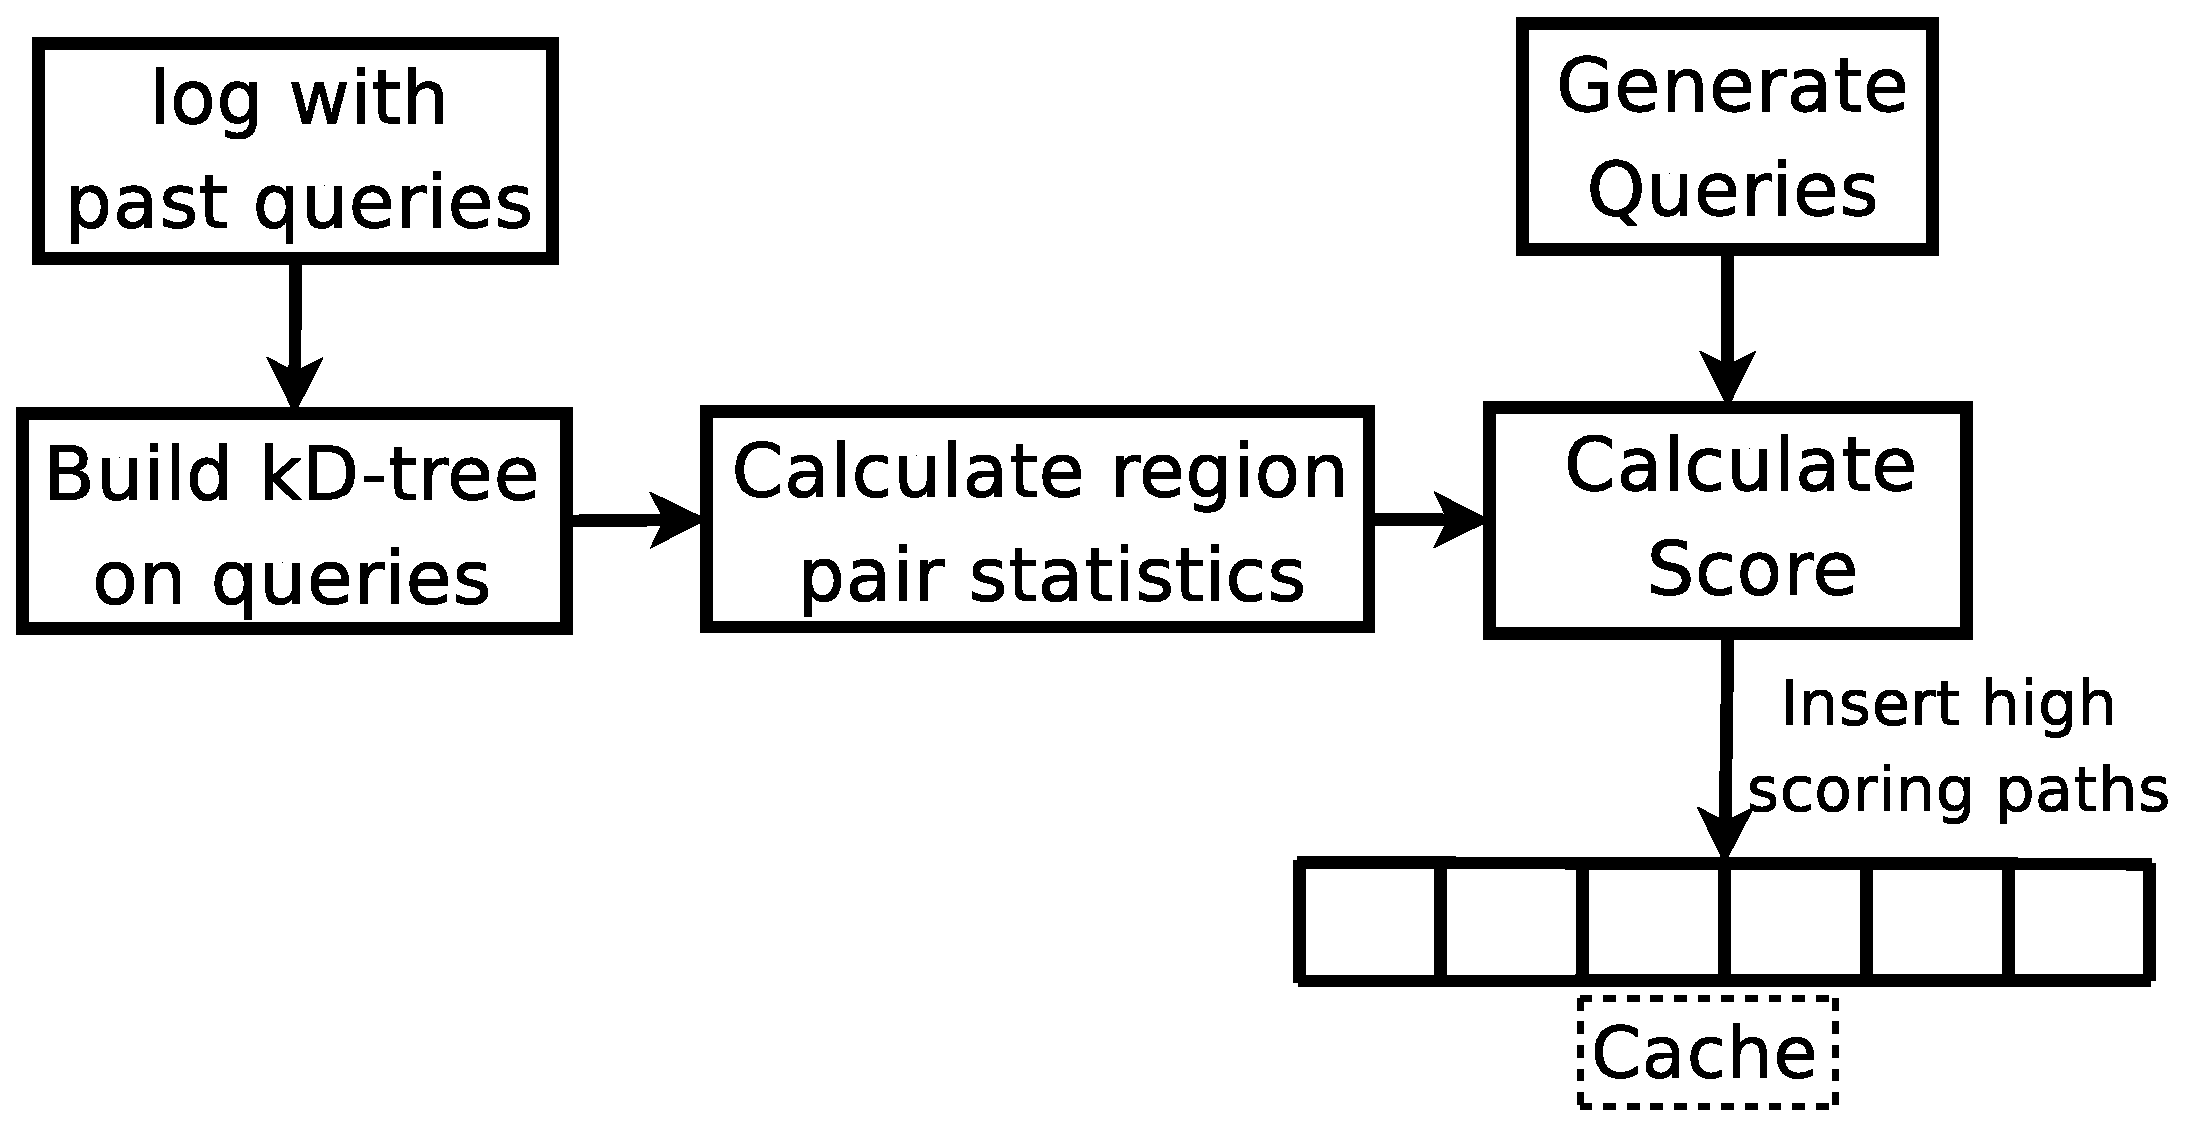
\includegraphics[width=0.5\textwidth]{figures/fillcache}
        \caption{Insertion of cache elements in offline phase.}
  \label{fig:fillcache}
\end{figure}


\subsection{Benefit model}

We will define our goals more formally, introducing the benefit equations we aim to minimize.

A query is a pair of vertice ids $(v_s, v_t)$, denoted $Q_{s,t}$ and the \spath returned from such query we denote $SP_{s,t}$. 
In order to evaluate goal \ref{item:goal3} we calculate the utility of the content in the cache, denoted $\tau$. To calculate $\tau$ we find the set of unique sub-paths from all \spaths in the cache ($\zeta$) and sum up the frequency, $\chi_{s,t}$, of each unique sub-path.

In order to evaluate our method we try to maximize $\tau$ (Eq. \ref{eq:benefit}).



\begin{equation} \label{eq:gamma}
 \gamma = \bigcup\limits_{\forall \spath \in \zeta} \Phi(\spath) \\
\end{equation}

\begin{equation} \label{eq:benefit}.
\tau = \sum\limits_{\forall SP_{s,t} \in \gamma} \chi_{s,t}
\end{equation}

\begin{equation} \label{eq:phi}
\Phi(sp) = \{ s \in sp, t \in sp, s \neq t : SP_{s,t} \}
\end{equation}


\begin{table}
\begin{tabular}{l l p{0.78\columnwidth}}
Q1:	&	$Q_{1,6} =$ 	& $\{v_1,v_3,v_4,v_5,v_6\}$\\
Q2:	&	$Q_{2,6} =$ 	& $\{v_2,v_3,v_4,v_5,v_6\}$ \\
Q3:	&	$Q_{1,4} =$ 	& $\{v_1,v_3,v_4\}$ \\
Q4:	&	$Q_{4,7} =$ 	& $\{v_4,v_5,v_7\}$ \\
Q5:	&	$Q_{2,5} =$ 	& $\{v_2,v_3,v_4,v_5\}$ \\
Q6:	&	$Q_{3,6} =$ 	& $\{v_3,v_4,v_5,v_6\}$ \\
\end{tabular}
\caption{Example Queries}
\label{tab:queries}
\end{table}

\begin{table}
\begin{tabular}{r p{0.78\columnwidth}}
$\Phi(SP_{1,6})=$ 	& $\{SP_{1,3},SP_{1,4},SP_{1,5},SP_{1,6},SP_{3,4},SP_{3,5},$\\
		 	& $SP_{3,6},SP_{4,5},SP_{4,6},SP_{5,6}\}$ \\
$\Phi(SP_{2,6})=$ 	& $\{SP_{2,3},SP_{2,4},SP_{2,5},SP_{2,6},SP_{3,4},SP_{3,5},$ \\
			& $SP_{3,6},SP_{4,5},SP_{4,6},SP_{5,6}\}$ \\
$\Phi(SP_{1,4})=$ 	& $\{SP_{1,3},SP_{1,4},SP_{3,4}\}$ \\
$\Phi(SP_{4,7})=$ 	& $\{SP_{4,5},SP_{4,7},SP_{5,7}\}$ \\
$\Phi(SP_{2,5})=$ 	& $\{SP_{2,3},SP_{2,4},SP_{2,5},SP_{3,4},SP_{3,5},SP_{4,5}\}$ \\
$\Phi(SP_{3,6})=$ 	& $\{SP_{3,4},SP_{3,5},SP_{3,6},SP_{4,5},SP_{4,6},SP_{5,6}\}$ \\\hline
$\gamma =$ 		& $\{SP_{1,3},SP_{1,4},SP_{1,5},SP_{1,6},SP_{3,4},SP_{3,5},$ \\
			& $SP_{3,6},SP_{4,5},SP_{4,6},SP_{5,6},SP_{2,3},SP_{2,4},SP_{2,5},$ \\
			& $SP_{2,6},SP_{4,5},SP_{4,7},SP_{5,7}\}$  \\
\end{tabular}
\caption{$\Phi$ (Eq. \ref{eq:phi}) results for queries in table \ref{tab:queries}}
\label{tab:phi}
\end{table}


% \begin{table}
% \center
% \begin{tabular}{rl|rl}
% $SP_{1,3}:$	& $\chi_{1,3} = 4$ & $SP_{1,4}:$	& $\chi_{1,4} = 2$ \\
% $SP_{1,5}:$	& $\chi_{1,5} = 3$ & $SP_{1,6}:$	& $\chi_{1,6} = 1$ \\
% $SP_{3,4}:$	& $\chi_{3,4} = 5$ & $SP_{3,5}:$	& $\chi_{3,5} = 8$ \\
% $SP_{3,6}:$	& $\chi_{3,6} = 7$ & $SP_{4,5}:$	& $\chi_{4,5} = 6$ \\
% $SP_{4,6}:$	& $\chi_{4,6} = 4$ & $SP_{5,6}:$	& $\chi_{5,6} = 2$ \\
% $SP_{2,3}:$	& $\chi_{2,3} = 4$ & $SP_{2,4}:$	& $\chi_{2,4} = 1$ \\
% $SP_{2,5}:$	& $\chi_{2,5} = 2$ & $SP_{2,6}:$	& $\chi_{2,6} = 3$ \\
% $SP_{4,7}:$	& $\chi_{4,7} = 5$ & $SP_{5,7}:$	& $\chi_{5,7} = 4$ \\
% \end{tabular}
% \caption{$\chi_{s,t}$ values for $\gamma$ in table \ref{tab:phi}}
% \label{tab:freq}
% \end{table}


\begin{table}
\center
\begin{tabular}{|l||l|l|l|l|l|l|l|}
\textbf{$\chi$ ${^s/_t}$}& \textbf{1}	& \textbf{2}	& \textbf{3}	& \textbf{4}	& \textbf{5}	& \textbf{6}	& \textbf{7} \\\hline
\textbf{1}	& X	&	& 4	& 2	& 3	& 1	&	 \\
\textbf{2}	& 	& X	& 4	& 1	& 2	& 3	&	 \\
\textbf{3}	& 4	& 4	& X	& 5	& 8	& 7	&	 \\
\textbf{4}	& 2	& 1	& 5	& X	& 6	& 4	& 5	 \\
\textbf{5}	& 3	& 2	& 8	& 6	& X	& 2	& 4	 \\
\textbf{6}	& 1	& 3	& 7	& 4	& 2	& X	&	 \\
\textbf{7}	&	&	&	& 5	& 4	&	& X	 \\
\end{tabular}
\caption{$\chi_{s,t}$ values for $\gamma$ in table \ref{tab:phi}}
\label{tab:freq}
\end{table}



When we want to evaluate the utility of $\zeta$ we first calculate $\gamma$ for each \spath. Table \ref{tab:phi} shows the set of sub-paths from the \spaths for each query Q1-Q6 from table \ref{tab:queries} (we assume all queries fit into the cache). Once we have all the sets of sub-paths from the cache content, we use equation \ref{eq:gamma} to union them together and obtain the set of unique sub-paths in the cache, $\gamma$ (see table \ref{tab:phi}). After we have obtained $\gamma$, we use equation \ref{eq:benefit} to calculate $\tau$, the total benefit we expect to have with the content in $\zeta$. With the $\gamma$ obtained, using $\chi_{s,t}$ values from table \ref{tab:freq}, $\tau$ would be 62 ($4+3+5+7+4+4+2+1+4+2+1+8+6+2+1+3+5 = 62$).

When filling the cache, during the offline phase, potential \spath items are scored based the sum of $\chi_{s,t}$-values from sub-paths not already present in the cache. If we assume Q1 is already in the cache and we are considering to insert either Q2 or Q4 next, then we first find the sub-paths for each query result, which is not already present in the cache. For Q2 it is $\{SP_{2,3},SP_{2,4},SP_{2,5},SP_{2,6}\}$ and for Q4 $\{SP_{4,7},SP_{5,7}\}$. When using the values for $\chi_{s,t}$ from table \ref{tab:freq} the utility of Q2 is $4+1+2+3=10$ and for Q4 $5+4=9$. In this case we would then insert Q2 as it represents the largest expected if inserted.

\subsection{Hardness Analysis}
Theoretical analysis showing how hard the problem is to solve for \spath caching.\\
show it is NP-Hard
 

\subsection{Greedy algorithm}
shows in more detail how we propose to solve our problem

\begin{algorithm}[H!bt]
\dontprintsemicolon
\SetVline

\SetKwInOut{Input}{input}\SetKwInOut{Output}{output}\SetKw{Return}{return}

\Input
{

	$G(V,E)$: Graph representation of Map \;
	$\Psi$: The cache \;
	$\mathcal{B}$: Cache budget \;
	
}
\vspace{0.7em}
\tcp{\emph{H Contains the utility score of all possible \spaths in $\mathbf{G(V,E)}$. The \spath is the value $v$ and the utility is the key $k$, $(k, v)$. The heap is sorted on the key.}}
H Initialize Max-Heap \;

\tcp{\emph{Initialially fill H}}

\ForAll{$\spath_{s,t} | s \in V, t \in V, s \neq t$} 
{
    H.push(S$(\chi, \spath_{s,t}, \Psi), \spath_{s,t}$) \;
}


\tcp{\emph{Fill cache}}
\While{$| \Psi | \leq \mathcal{B}$ AND $\spath_{ms}.k \neq 0$ OR $| H | > 0$}
{
	\tcp{\emph{Assign (utility,\spath) pair with the highest utility to $\spath_{ms}$}}
	$ \langle  key_{max},  SP_{max} \rangle \leftarrow$ H.pop() \; 
	\tcp{\emph{Update utility, as previous \spath insertion has changed it}}
	$key_{max} = S(\chi, \spath_{max}, \Psi)$
	\tcp{\emph{H.TopKey() looks at the top (k,v) pair without removing it from the heap}}
	\If{$key_{max} \geq H.TopKey$} 	
	{
	    \If{$( \mathcal{B} - | \Psi | ) \geq | \spath_{max} |$}
	    {
		$\Psi.insert(\spath_{max})$\;
	    }
	}
	\Else
	{
	    H.push(S$(\chi, \spath_{max}, \Psi), \spath_{max}$) \;
	}
}

\caption{\salgons($G(V,E), \Psi, \mathcal{B}$)}
\label{alg:greedy}
\end{algorithm}

\subsection{Statistics extraction}

\subsubsection{Partition map} 
solves goal 1. reduce time on \spath calculation as it aids the cache with information on which paths may be useful.\\ 
discussion of kD-Tree.

\begin{algorithm}[H!bt]
\dontprintsemicolon
\SetVline

\SetKwInOut{Input}{input}\SetKwInOut{Output}{output}\SetKw{Return}{return}



\Input{
	$\mathbf{\spath_{s,t}}$: A \spath.\;
}

\Output{
	An integer representing the score
}



 \funcc{Score}{\spath_{s,t}}
{
	\textbf{H}.push($S(\chi, SP_{s,t}, \Psi), SP_{s,t}$) \;
% 	\ForEach{edge $e \in \alpha.t$}
% 	{
% 		\ForEach {$psr \in PS$ }
% 		{
% 			\If{$e \in psr.p_{edges}$}
% 			{
% 				${\poins}cand \leftarrow {\poins}cand \cup psr$\;
% 			}
% 		} 
% 	}
}

\caption{Score() function using statistics}
\label{alg:score}
\end{algorithm}

\subsection{Cache representations and cache concepts} \label{subsec:cacherepresentatons}
How the cache is stored, and how we search it, is crucial to the performance of a cache. We will present the basic, naive, approach as well as 3 ideas for improvement.

\subsubsection{Simple array of paths}% - baseline for goal 2, unoptimized and expensive to use.
The simplest way to represent a cache is a simple array of paths. This representation will we expensive to search since we may need to search all paths in the cache, akin to a double for loop, every time we want to check if an item is in the cache.

If we have a cache with $SP_{1,6},SP_{2,6},$ and $SP_{1,4}$ already in the cache and $Q_{4,7}$ is received, then we need to search the cache to see if we can get a cache hit. Since there can be no cache hit for $Q_{4,7}$ we need to scan all nodes for all paths, which would be 13 in this example (length of $SP_{1,6},SP_{2,6},$, $SP_{1,4}$, see table \ref{tab:queries}).

We will use this representation as the baseline for goal 2 when comparing the improvement when using any of the following cache representation ideas.

\subsubsection{Simple array of paths inverted list} - solves goal 2, reduces the query time of the cache.\\
A simple, yet very effective, way to improve the search time of a cache represented by a simple array is to add an inverted list on top of the cache. We add an inverted list with node ids as keys and values being a list of array indices which holds paths containing specific node ids. By using such an inverted list we just need to do the intersection between the lists retrieved by querying the inverted list with the start and target node ids. 


\textbf{*example*}

\subsubsection{Graph representation} - solves goal 1, allows for more paths in cache, which should translate more cache hits.

\subsubsection{Sharing sub-paths} - solves goal 1, allows for more paths in cache, translating to more cache hits. Unfortunately has a negative impact on goal 2 as it introduces some overhead in query time.

